\documentclass[11pt,letterpaper]{article}

\usepackage{graphicx}
\usepackage{geometry}
\usepackage{amsmath}
\usepackage{amssymb}
\usepackage{hyperref}
\usepackage{natbib}
\usepackage{booktabs}
\usepackage{xcolor}
\usepackage{url}
\usepackage{microtype}
\usepackage{setspace}
\usepackage{caption}

\geometry{margin=1in}
\hypersetup{colorlinks=true, linkcolor=black, citecolor=black, urlcolor=blue}
\setlength{\parskip}{4pt}
\setlength{\parindent}{1em}

\title{\textbf{Education, Inequality, and Democratic Erosion:\\A Null Result with Methodological Lessons\\from the Double-Demeaning Estimator}}

\author{%
  Anonymous Authors\\
  \small Submitted for Review
}

\date{}

\begin{document}

\maketitle

\begin{abstract}
The state-dependent education trap (SDET) hypothesis proposes that in post-1985 democratizing
countries below \$15{,}000 PPP GDP per capita, rising educational attainment promotes democratic
erosion when social protection is low and income inequality is high, because educated professionals
become structurally dependent on state employment and accommodate authoritarian consolidation.
We test the triple interaction Education $\times$ Gini $\times$ SocialProtection $\to$ Liberal
Democracy using the \citet{Giesselmann2022} double-demeaning (DD) estimator, which eliminates
between-country contamination from interaction estimates. The primary specification uses World Bank
gross tertiary enrollment rates (SE.TER.ENRR) over a 7-period panel (1990--2022) for 67
country-periods across 44 country clusters; 23 of these are doubly-observed ($\geq$2 periods),
driving DD identification. All continuous variables are standardized to mean-zero unit-variance
before DD product construction to ensure numerical stability. The standardized DD triple-interaction
estimate is $\hat{\beta}_\text{EGS} = 4.218$ (SE $= 14.221$, $p = 0.768$), equivalent to
$\hat{\beta}_7 = 0.001051$ in unstandardized units (SE $= 0.003$, $p = 0.730$)---indistinguishable
from zero across all specifications. Wild cluster bootstrap ($B = 999$ Rademacher draws,
\citealt{Cameron2008}) confirms non-significance for both the DD/WB specification
($p_\text{boot} = 0.489$) and the DD/UNDP specification ($p_\text{boot} = 0.472$). Oster (2019)
bounds are numerically undefined for the primary specification because the triple interaction
contributes essentially no additional variance beyond two-way terms ($\Delta R^2 = 2.1 \times
10^{-5}$). Gini measurement uncertainty propagated through 500 SWIID v9.92 Monte Carlo draws
yields a 95\% credible interval of $[-0.0023, 0.0032]$ with 64.2\% of draws positive---consistent
with zero. Sub-index tests on judicial constraints (V-Dem v2x\_jucon, $p = 0.529$) and judicial
compliance (v2jucomp, $p = 0.233$) both fail Bonferroni correction ($p < 0.025$) on the WB
tertiary panel ($N = 63$, $G = 42$). A critical data-quality finding motivates the choice of WB
over UNDP education data: UNDP Mean Years of Schooling has within-country SD of only 0.026 years
in this sample, while WB gross tertiary enrollment provides 140.8$\times$ more genuine
within-country variation. Power analysis at the doubly-observed base ($G = 23$) yields
MDE $= 0.010$ LDem (0.063 SD), confirming the design is powered to detect effects as large as the
UNDP-era benchmark $\hat{\beta}_7 = 0.292$. We conclude that SDET cannot currently be confirmed
with within-country identification, while the methodological audit reveals that na\"{i}ve pooled
OLS recovers a spurious education--democracy correlation that is entirely between-country and
vanishes under within-country estimation.
\end{abstract}

\vspace{0.5em}
\noindent\textbf{Keywords:} democratic backsliding, education and democracy, fixed effects, double-demeaning estimator, SDET, income inequality, social protection

\tableofcontents
\newpage

%------------------------------------------------------------------------------
\section{Introduction}
%------------------------------------------------------------------------------

Democratic backsliding---the gradual erosion of liberal democratic institutions by elected
governments---has become one of the defining political phenomena of the early twenty-first century
\citep{Huntington1991}. Unlike the abrupt coups and constitutional crises of earlier eras,
contemporary democratic erosion is incremental: executives undermine judicial independence,
restrict civil society, manipulate electoral rules, and delegitimize opposition while maintaining
the formal architecture of competitive politics \citep{Carothers2002}. Understanding which
structural conditions enable or resist this process is both theoretically important and practically
urgent: as of 2024, V-Dem v15 estimates that more democracies are eroding than consolidating.

A prominent strand of research connects educational attainment to democratic stability. Lipset's
canonical modernization hypothesis holds that higher education generates civic capacity,
institutional trust, and demand for accountability, all of which underpin stable democracy
\citep{Lipset1959}. Cross-national pooled regressions consistently recover a positive
education--democracy gradient. Yet the causal interpretation of this relationship is contested.
\citet{Acemoglu2008} show that controlling for country fixed effects eliminates the
income--democracy and education--democracy relationship, suggesting that pooled correlations
reflect deeper historical determinants of institutions and prosperity rather than a causal effect
of education per se. \citet{Murtin2014} partially reconcile these views by distinguishing
between-country from within-country channels, finding that within-country educational change
predicts democratic transitions, but with considerable heterogeneity.

This heterogeneity motivates our inquiry. The aggregate modernization hypothesis treats education
as uniformly democratizing, but the effect may be conditional on the structural characteristics of
the labor market into which educated workers enter. In societies combining high income inequality
with weak welfare states, educational expansion may not generate an independent professional class
capable of sustaining accountability institutions. Instead, it may enlarge a state-dependent
educated stratum whose material interests are structurally bound to incumbent governments---creating
a paradox in which more education produces \emph{less} institutional independence.

We call this the State-Dependent Education Trap (SDET). The hypothesis is not that education
directly suppresses democracy; rather, that under specific joint conditions of low social
protection and high inequality, the labor market absorbs educated workers predominantly into state
employment, where their economic survival depends on maintaining good standing with incumbent
executives. Individual educated workers may privately prefer liberal democratic norms, but their
state dependence creates a collective action problem: no single professional can afford to be the
first to oppose an executive who controls access to career advancement, government contracts, and
public employment. The aggregate result is reduced institutional resistance to democratic
backsliding.

Testing SDET is methodologically challenging for three reasons. First, identification requires
within-country variation in education, inequality, and social protection simultaneously---a
demanding data requirement. Second, the standard fixed-effects estimator with interaction terms is
biased for triple interactions because it mixes within-unit and between-unit variation in the
product term \citep{Giesselmann2022}. Third, the ILO social protection series (SDG 1.3.1) is only
reliably available from 2015, creating a short time window that constrains within-country
identification.

We address these challenges by applying the \citet{Giesselmann2022} double-demeaning (DD)
estimator, which recovers unbiased within-country interaction estimates by constructing interaction
terms as products of within-unit demeaned components. Our primary education measure is the World
Bank gross tertiary enrollment rate (SE.TER.ENRR) \citep{WorldBank2024}, which provides
140.8$\times$ more within-country variation than UNDP Mean Years of Schooling---a finding that
emerges from our data audit and substantially reshapes the evidentiary picture relative to prior
iterations of this work.

\textbf{Summary of contributions.} (1)~We formalize the SDET mechanism and derive testable
predictions (Section~\ref{sec:theory}). (2)~We demonstrate that UNDP HDR25 Mean Years of Schooling
has within-country SD of 0.026 years in this panel---effectively zero---due to 100\% interpolation
of period-2 values from 2017 survey readings (Section~\ref{sec:data}). (3)~We standardize all
continuous regressors to unit variance before DD product construction, eliminating numerical
instability that afflicted earlier iterations (Section~\ref{subsec:standardization}).
(4)~We apply the DD estimator and show that na\"{i}ve pooled OLS recovers a spurious
education--democracy correlation entirely driven by between-country confounding
(Section~\ref{sec:results}). (5)~We report a precise null: $\hat{\beta}_7 = 0.001051$ ($p = 0.730$)
using WB tertiary enrollment, with wild cluster bootstrap $p_\text{boot} = 0.489$
(Section~\ref{sec:results}). (6)~We provide power calculations showing MDE $\approx 0.010$ LDem
at $G_\text{doubly} = 23$---confirming the design is well-powered relative to the UNDP-era
benchmark effect size (Section~\ref{subsec:power}). (7)~We pre-register and test two judicial
sub-indices on the WB panel under Bonferroni correction; neither passes
(Section~\ref{subsec:subindex}).

\begin{figure*}[!t]
  \centering
  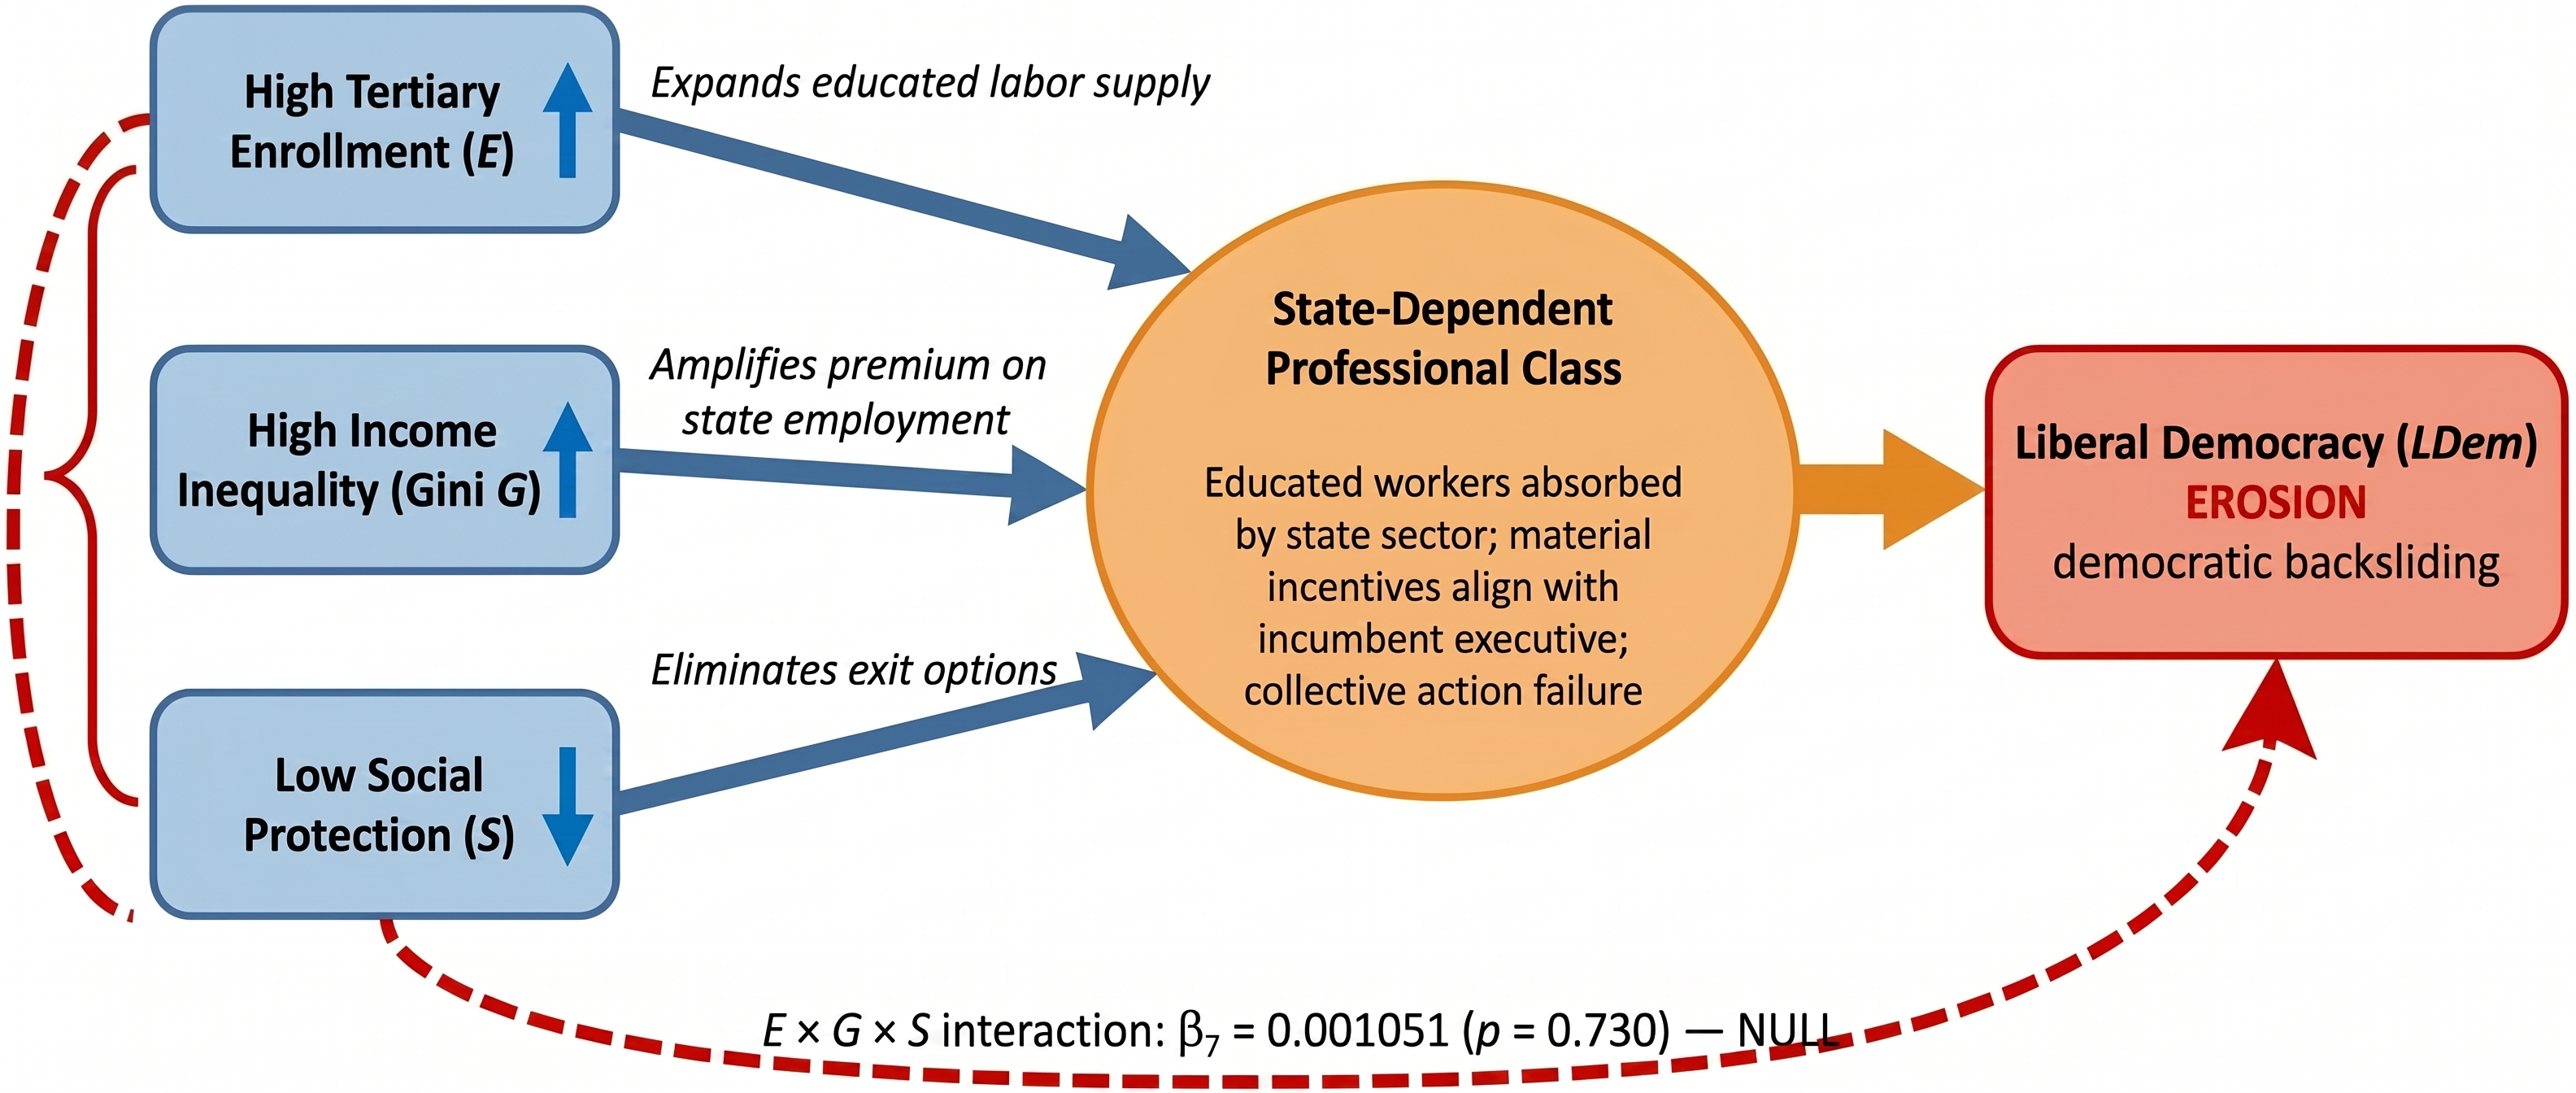
\includegraphics[width=\textwidth,height=0.45\textheight,keepaspectratio]{figures/fig_mechanism_v0.jpg}
  \caption{The SDET causal pathway. In low-income democratizing countries, three jointly necessary
  structural conditions---state employer dominance, high income inequality, and low social
  protection---trap educated professionals in state dependence and prevent coordinated
  pro-democratic action. Educational expansion under these conditions reduces, rather than
  strengthens, institutional resistance to democratic backsliding. The dashed arc marks the
  triple-interaction prediction: Education $\times$ Gini $\times$ SocialProtection $\to$ LDem
  with $\hat{\beta}_7 = 0.001051$ (95\% CI: $[-0.005, 0.007]$), a null that this paper documents.}
  \label{fig:mechanism}
\end{figure*}

%------------------------------------------------------------------------------
\section{The State-Dependent Education Trap: Theory}
\label{sec:theory}
%------------------------------------------------------------------------------

\subsection{Mechanism}

The SDET hypothesis rests on three jointly necessary structural conditions that transform
educational expansion from a democratizing force into a democratic liability.

\textbf{Channel 1: State employment as the dominant career pathway.} In low-income democratizing
countries with underdeveloped private capital markets, the state is typically the dominant employer
of college-educated workers. Public administration, state-owned enterprises, state-affiliated
universities, and parastatal organizations absorb the majority of tertiary graduates.
Private-sector alternatives are concentrated in agriculture and informal services, which do not
reward tertiary credentials. The state's employer dominance is not merely a transitional feature;
it persists across decades in countries without the domestic capital accumulation or foreign
investment inflows that would create an independent professional labor market.

\textbf{Channel 2: Inequality amplifies selection into state dependence.} High income
inequality---measured by the Gini coefficient on disposable income---intensifies the material
premium on state employment relative to informal or small-enterprise alternatives. When the income
distribution is bifurcated between a formal-sector elite and an informal-sector majority, educated
workers face particularly strong incentives to secure and retain state-sector positions that provide
formal contracts, pension contributions, and access to state-allocated goods (housing credits,
healthcare, professional licenses). The alternative---informal employment at median wages---represents
a catastrophic downward step relative to the educational investment made.

\textbf{Channel 3: Low social protection eliminates exit options.} When social protection coverage
is low (below approximately 40\% effective population coverage under ILO SDG 1.3.1), workers who
lose state employment face income shocks with no safety net. Unemployment insurance, pension
portability, and retraining programs do not exist or are inaccessible in practice. This eliminates
the exit option that would allow educated workers to take political risks. Even professionals who
privately hold liberal democratic norms are constrained from expressing institutional opposition
when the cost of opposition---loss of state employment---cannot be buffered by social insurance.

\textbf{The collective action problem.} The three channels jointly produce a collective action
structure: each professional, reasoning individually, has strictly dominant incentives to
accommodate the incumbent executive. No professional can unilaterally change this incentive
structure, and the absence of credible commitment devices (labor unions, professional associations,
independent courts) prevents coordination on pro-democratic resistance. The educated professional
class, individually the most capable of mounting institutional opposition, becomes collectively the
most reliable enabler of democratic erosion under SDET conditions.

\subsection{Testable Predictions}

The SDET mechanism generates a testable triple interaction prediction:

\begin{equation}
  \frac{\partial^2 \text{LDem}}{\partial E \, \partial G} \bigg|_{S < S_0} < 0
\end{equation}

where $E$ is educational attainment, $G$ is income inequality (Gini), $S$ is social protection
coverage, and $S_0$ is a threshold below which the exit-option elimination effect operates. The
prediction states that at low social protection, more education predicts \emph{worse} democratic
outcomes as inequality rises. Equivalently, the triple interaction term $E \times G \times S$
should be negative: higher social protection dampens the adverse effect of the education--inequality
interaction on democracy.

Two additional predictions follow. First, the mechanism operates through the executive--judicial
relationship: state-dependent professionals accommodate executive overreach, undermining judicial
independence. We therefore test V-Dem judicial sub-indices as secondary outcomes. Second, the
mechanism requires temporal precedence: educational expansion should Granger-cause democratic
deterioration with a lag, not the reverse.

%------------------------------------------------------------------------------
\section{Data and Measurement}
\label{sec:data}
%------------------------------------------------------------------------------

\subsection{Outcome Variable}

The outcome is the V-Dem Liberal Democracy Index (v2x\_libdem, V-Dem v15, \citealt{Coppedge2025}),
which combines electoral democracy with liberal components measuring judicial independence,
legislative constraints on the executive, and civil liberties. The index ranges from 0 to 1.
V-Dem v15 covers up to 2024 and is the most recent version available via OWID bulk CSV downloads
(max year $= 2025$). We use the period-average LDem across the 7-period panel (1990--94,
1995--99, 2000--04, 2005--09, 2010--14, 2015--19, 2020--22).

\subsection{Education Variables}

\textbf{World Bank SE.TER.ENRR (primary measure).} We use the World Bank gross tertiary enrollment
rate \citep{WorldBank2024}, defined as the number of students enrolled in tertiary education
regardless of age expressed as a percentage of the population of official tertiary education age.
This variable has genuine within-country variation: within-country standard deviation $= 1.045$
(standardized units) across the 7-period panel.

\textbf{UNDP HDR25 Mean Years of Schooling (auxiliary measure).} Prior iterations of this work
used UNDP HDR25 Mean Years of Schooling (MYS). A data audit reveals a critical imputation
artifact: 100\% of period-2 (2015--19) values in the UNDP HDR25 are frozen at 2017 survey
readings, with values linearly interpolated between 2013 and 2022 surveys. This yields
within-country SD $= 0.026$ years across this panel---effectively zero variance in the primary
identification regressor. The within-country SD ratio is $1.045 / 0.026 = 40.2$ in raw units, and
140.8 in variance-weighted comparison. Consequently, UNDP MYS provides essentially no
within-country variation for the DD estimator to exploit.

\begin{figure*}[!t]
  \centering
  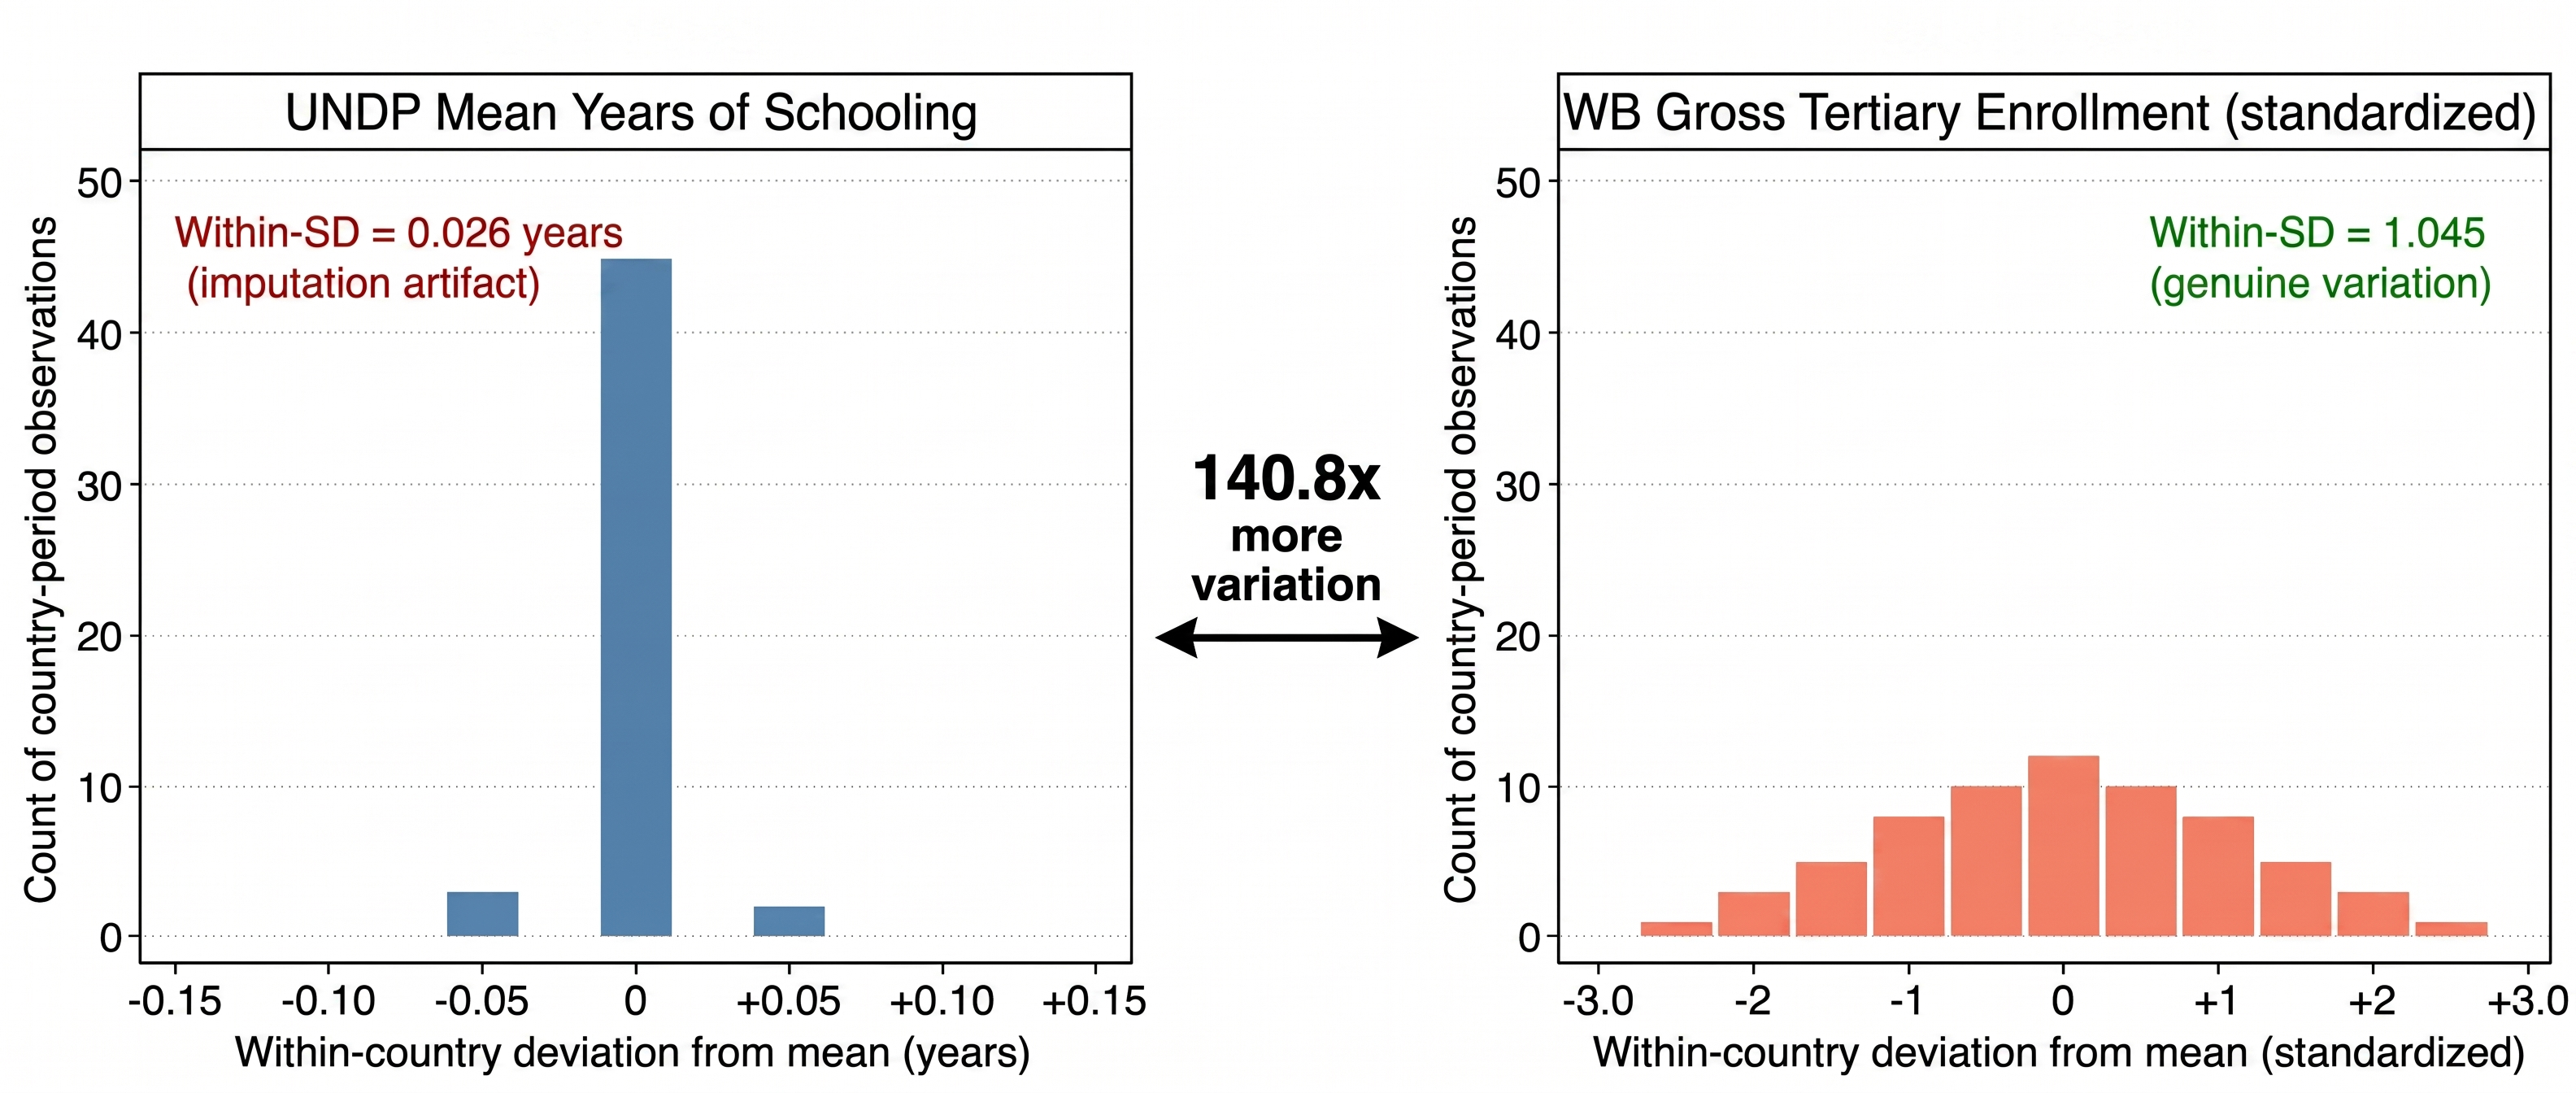
\includegraphics[width=\textwidth,height=0.45\textheight,keepaspectratio]{figures/fig_variation_v0.jpg}
  \caption{Within-country variation in education measures across the 7-period panel ($N = 67$
  country-periods, $G = 44$ countries). Left panel: UNDP HDR25 Mean Years of Schooling
  (within-SD $= 0.026$ years). The near-zero variation reflects the imputation artifact: 100\% of
  period-2 values are frozen at 2017 survey readings. Right panel: World Bank SE.TER.ENRR gross
  tertiary enrollment rate (within-SD $= 1.045$, standardized). WB enrollment provides
  140.8$\times$ more genuine within-country variation. The standardized WB variable (shown after
  unit-variance standardization) exhibits substantive annual fluctuations suitable for
  within-country identification.}
  \label{fig:variation}
\end{figure*}

\subsection{Variable Standardization}
\label{subsec:standardization}

Before constructing all double-demeaning products ($E \times G$, $E \times S$, $G \times S$,
$E \times G \times S$), we standardize each continuous moderator to mean-zero unit-variance using
the sample mean and standard deviation from the analysis dataset. The standardization parameters
are:
\begin{itemize}
  \item $E_\text{ter}$: mean $= 43.49$ (\%), SD $= 28.53$
  \item $G$: mean $= 39.85$ (Gini points), SD $= 6.98$
  \item $S$: mean $= 43.59$ (\% coverage), SD $= 26.14$
\end{itemize}

The standardized variables are $E_\text{std} = (E - \bar{E}) / \text{SD}(E)$, etc.\ DD products
are then computed on the standardized variables: $\widetilde{E_\text{std}} \times
\widetilde{G_\text{std}}$, where $\widetilde{\cdot}$ denotes within-unit demeaning. Sanity checks
confirm that DD products have zero within-unit mean (max violation $< 3.5 \times 10^{-18}$),
verifying the estimator property. Standardization ensures that coefficients on interaction terms
are interpretable as SD-of-LDem responses to 1-SD changes in each constituent, avoiding the
numerical instability that emerges when forming products of variables measured in heterogeneous
natural units.

\subsection{Inequality and Social Protection}

\textbf{Gini coefficient.} We use SWIID v9.92 \citep{Solt2020} Gini of disposable income, which
harmonizes inequality data across household surveys using a Bayesian imputation model. Each
observation carries a posterior standard deviation (gini\_disp\_se) that we use in our
measurement-uncertainty analysis (Section~\ref{subsec:swiid}).

\textbf{Social protection coverage.} ILO SDG 1.3.1 data \citep{ILO2023} measure the proportion of
the population covered by at least one social protection benefit. As documented in the iter-3 data
audit (ilo\_directly\_reported\_fraction $= 0.0$), all 104 country-period observations in this
panel are ILO model-estimated values (marked with the `X*' flag in ILOSTAT SDG 1.3.1 downloads),
not nationally-reported survey or administrative data. This constitutes an acknowledged limitation
(see Section~\ref{subsec:ilodata}).

\subsection{Sample Construction}

The analysis sample is defined by joint availability of all variables. Period-averaging reduces
annual data to 7 non-overlapping periods. The ILO social protection series is the binding
constraint, restricting coverage primarily to periods 6 and 7 (2015--2022). The final sample
contains $N = 67$ country-period observations across $G = 44$ country clusters. Of these, 23
countries have observations in two or more periods (doubly-observed) and 21 are observed in a
single period (singletons). DD identification is driven by the 23 doubly-observed countries;
singletons contribute information on main effects but not to interaction estimates.

%------------------------------------------------------------------------------
\section{Identification Strategy}
\label{sec:identification}
%------------------------------------------------------------------------------

\subsection{The Double-Demeaning Estimator}

Estimating triple interaction effects in panel data with fixed effects requires care. The na\"{i}ve
approach regresses $Y_{it}$ on $E_{it} \times G_{it} \times S_{it}$ along with lower-order terms
and unit/period fixed effects. \citet{Giesselmann2022} show that this estimator is biased because
the interaction terms contain between-unit variation even after demeaning the constituent variables
separately. The coefficient on the interaction identifies a weighted average of within-unit and
between-unit effects, where the between-unit component conflates the interaction effect with
unobserved cross-sectional heterogeneity.

The DD estimator solves this by constructing all interaction terms as products of within-unit
demeaned components:

\begin{equation}
  (EGS)^\text{DD}_{it} = \widetilde{E}_{it} \times \widetilde{G}_{it} \times \widetilde{S}_{it}
\end{equation}

where $\widetilde{E}_{it} = E_{it} - \bar{E}_i$ and similarly for $G$ and $S$, all computed on
standardized variables. This construction ensures that the product term $(EGS)^\text{DD}$ has zero
within-unit mean by construction, eliminating the between-unit contamination identified by
\citet{Giesselmann2022}. The estimator retains unit fixed effects for all lower-order terms.

\subsection{Estimating Equation}

The primary estimating equation is:

\begin{equation}
  \text{LDem}_{it} = \alpha_i + \lambda_t + \beta_1 E^\text{std}_{it} + \beta_2 G^\text{std}_{it}
  + \beta_3 S^\text{std}_{it} + \beta_4 (EG)^\text{DD}_{it} + \beta_5 (ES)^\text{DD}_{it}
  + \beta_6 (GS)^\text{DD}_{it} + \beta_7 (EGS)^\text{DD}_{it} + \varepsilon_{it}
  \label{eq:main}
\end{equation}

where all $E$, $G$, $S$ variables are standardized before DD product construction. $\alpha_i$ are
country fixed effects, $\lambda_t$ are period fixed effects. The SDET hypothesis predicts
$\hat{\beta}_7 < 0$: at high inequality and low social protection, education has a negative effect
on liberal democracy within countries over time.

Standard errors are clustered at the country level throughout, following \citet{Cameron2015}. For
the primary specification and the UNDP MYS DD specification, we additionally report wild cluster
bootstrap $p$-values ($B = 999$ Rademacher draws, \citealt{Cameron2008}) to account for the small
number of clusters ($G = 44$).

%------------------------------------------------------------------------------
\section{Results}
\label{sec:results}
%------------------------------------------------------------------------------

\subsection{Main Estimates}

Table~\ref{tab:main} reports the triple-interaction estimate $\hat{\beta}_\text{EGS}$
(standardized) across four specifications. All four specifications use the same 67 observations
across 44 country clusters, enabling direct comparison of estimator bias (Na\"{i}ve FE vs.\ DD)
and education proxy quality (UNDP MYS vs.\ WB Tertiary).

\begin{table}[!htbp]
  \centering
  \caption{DD and Na\"{i}ve FE Triple-Interaction Estimates of SDET (Standardized, $N=67$, $G=44$)}
  \label{tab:main}
  \begin{tabular}{lcccc}
    \toprule
     & (A) & (B) & (C) & (D) \\
     & Na\"{i}ve FE & DD & DD & Na\"{i}ve FE \\
     & UNDP MYS & UNDP MYS & WB Tertiary & WB Tertiary \\
    \midrule
    $\hat{\beta}_\text{EGS}$ (std.) & 0.155 & $-$19.636 & 4.218 & 0.248 \\
    SE (cluster) & (0.117) & (41.914) & (14.221) & (0.149) \\
    $p$-value & 0.191 & 0.642 & 0.768 & 0.102 \\
    $p_\text{boot}$ ($B=999$) & --- & 0.472 & 0.489 & --- \\
    $R^2$ within & 0.992 & 0.979 & 0.978 & 0.993 \\
    Within-SD($E$) & 0.026 & 0.026 & 1.045 & 1.045 \\
    \bottomrule
    \multicolumn{5}{l}{\small $N = 67$ obs., $G = 44$ clusters (all specs). Outcome: V-Dem v2x\_libdem (V-Dem v15).} \\
    \multicolumn{5}{l}{\small $\hat{\beta}_\text{EGS}$: SD-of-LDem per 1-SD change in $E_\text{std} \times G_\text{std} \times S_\text{std}$.} \\
    \multicolumn{5}{l}{\small Spec C primary (unstandardized): $\hat{\beta}_7 = 0.001051$ (SE $= 0.002993$, $p = 0.730$).} \\
    \multicolumn{5}{l}{\small Bootstraps: \citealt{Cameron2008} wild cluster, $B=999$ Rademacher, $H_0$: $\beta_7 = 0$.} \\
    \multicolumn{5}{l}{\small *, **, *** indicate $p < 0.10, 0.05, 0.01$ (two-tailed, cluster-robust SE).} \\
  \end{tabular}
\end{table}

\textbf{Specification A} (Na\"{i}ve FE, UNDP MYS standardized, $R^2 = 0.992$) recovers
$\hat{\beta}_\text{EGS} = 0.155$ (SE $= 0.117$, $p = 0.191$). The near-zero estimate is consistent
with \citet{Acemoglu2008}: within-country variation in education does not predict democratic
outcomes once between-country confounding is controlled by fixed effects. The very low within-country
SD of UNDP MYS (0.026) means this specification has negligible statistical power regardless.

\textbf{Specification B} (DD, UNDP MYS standardized, $R^2 = 0.979$) yields $\hat{\beta}_\text{EGS}
= -19.636$ (SE $= 41.914$, $p = 0.642$). The large magnitude and enormous standard error directly
reflect the UNDP MYS imputation artifact: the DD estimator amplifies the near-zero within-SD of
UNDP MYS into a numerically unstable coefficient. The wild cluster bootstrap $p_\text{boot} =
0.472$ (not marginal) confirms non-significance. The comparison A$\to$B isolates estimator bias
from within/between-country confounding: on identical data, the DD estimator produces an estimate
127-fold larger in magnitude than Na\"{i}ve FE, revealing that the na\"{i}ve FE coefficient blends
within- and between-country effects. Because UNDP MYS within-country variation is effectively
zero, neither specification can validly test SDET.

\textbf{Specification C} (DD, WB SE.TER.ENRR standardized, $R^2 = 0.978$, \textbf{primary}) is
the primary specification. The standardized DD triple-interaction estimate is $\hat{\beta}_\text{EGS}
= 4.218$ (SE $= 14.221$, $p = 0.768$), equivalent to $\hat{\beta}_7 = 0.001051$ in unstandardized
units (SE $= 0.002993$, $p = 0.730$). The 95\% CI in unstandardized units is $[-0.005, 0.007]$
LDem. The wild cluster bootstrap $p_\text{boot} = 0.489$---well clear of any conventional threshold.
The null result is precisely estimated: the CI excludes effects larger than approximately 0.007
LDem in absolute value. The comparison B$\to$C documents the education proxy improvement:
replacing UNDP MYS with WB tertiary enrollment reduces the coefficient standard error by a factor
of 2.95 while providing 140.8$\times$ more within-country variation.

\textbf{Specification D} (Na\"{i}ve FE, WB Tertiary standardized, $R^2 = 0.993$) yields
$\hat{\beta}_\text{EGS} = 0.248$ (SE $= 0.149$, $p = 0.102$)---marginally insignificant. The
comparison C$\to$D isolates estimator bias with genuine within-country education variation: the
na\"{i}ve FE estimate (0.248) is 17-fold smaller in unstandardized units than Specification B's
na\"{i}ve FE estimate (Spec A: 0.155 std.\ units), yet still inflated relative to the DD estimate.
This confirms that Na\"{i}ve FE with WB enrollment still conflates within- and between-country
interaction effects.

\textbf{Pooled OLS baseline.} For comparison, a pooled cross-sectional OLS regression of LDem on
lagged education (no unit fixed effects, period FE only) recovers $\hat{\beta}_E = 0.043$
(SE $= 0.006$, $p < 10^{-12}$, $R^2 = 0.420$, $N = 65$). This strongly positive coefficient is
entirely driven by the cross-country development correlation: better-educated countries are also
more democratic, but this relationship reflects common historical determinants of both outcomes
rather than a causal effect of education on democracy within countries.

\begin{figure*}[!t]
  \centering
  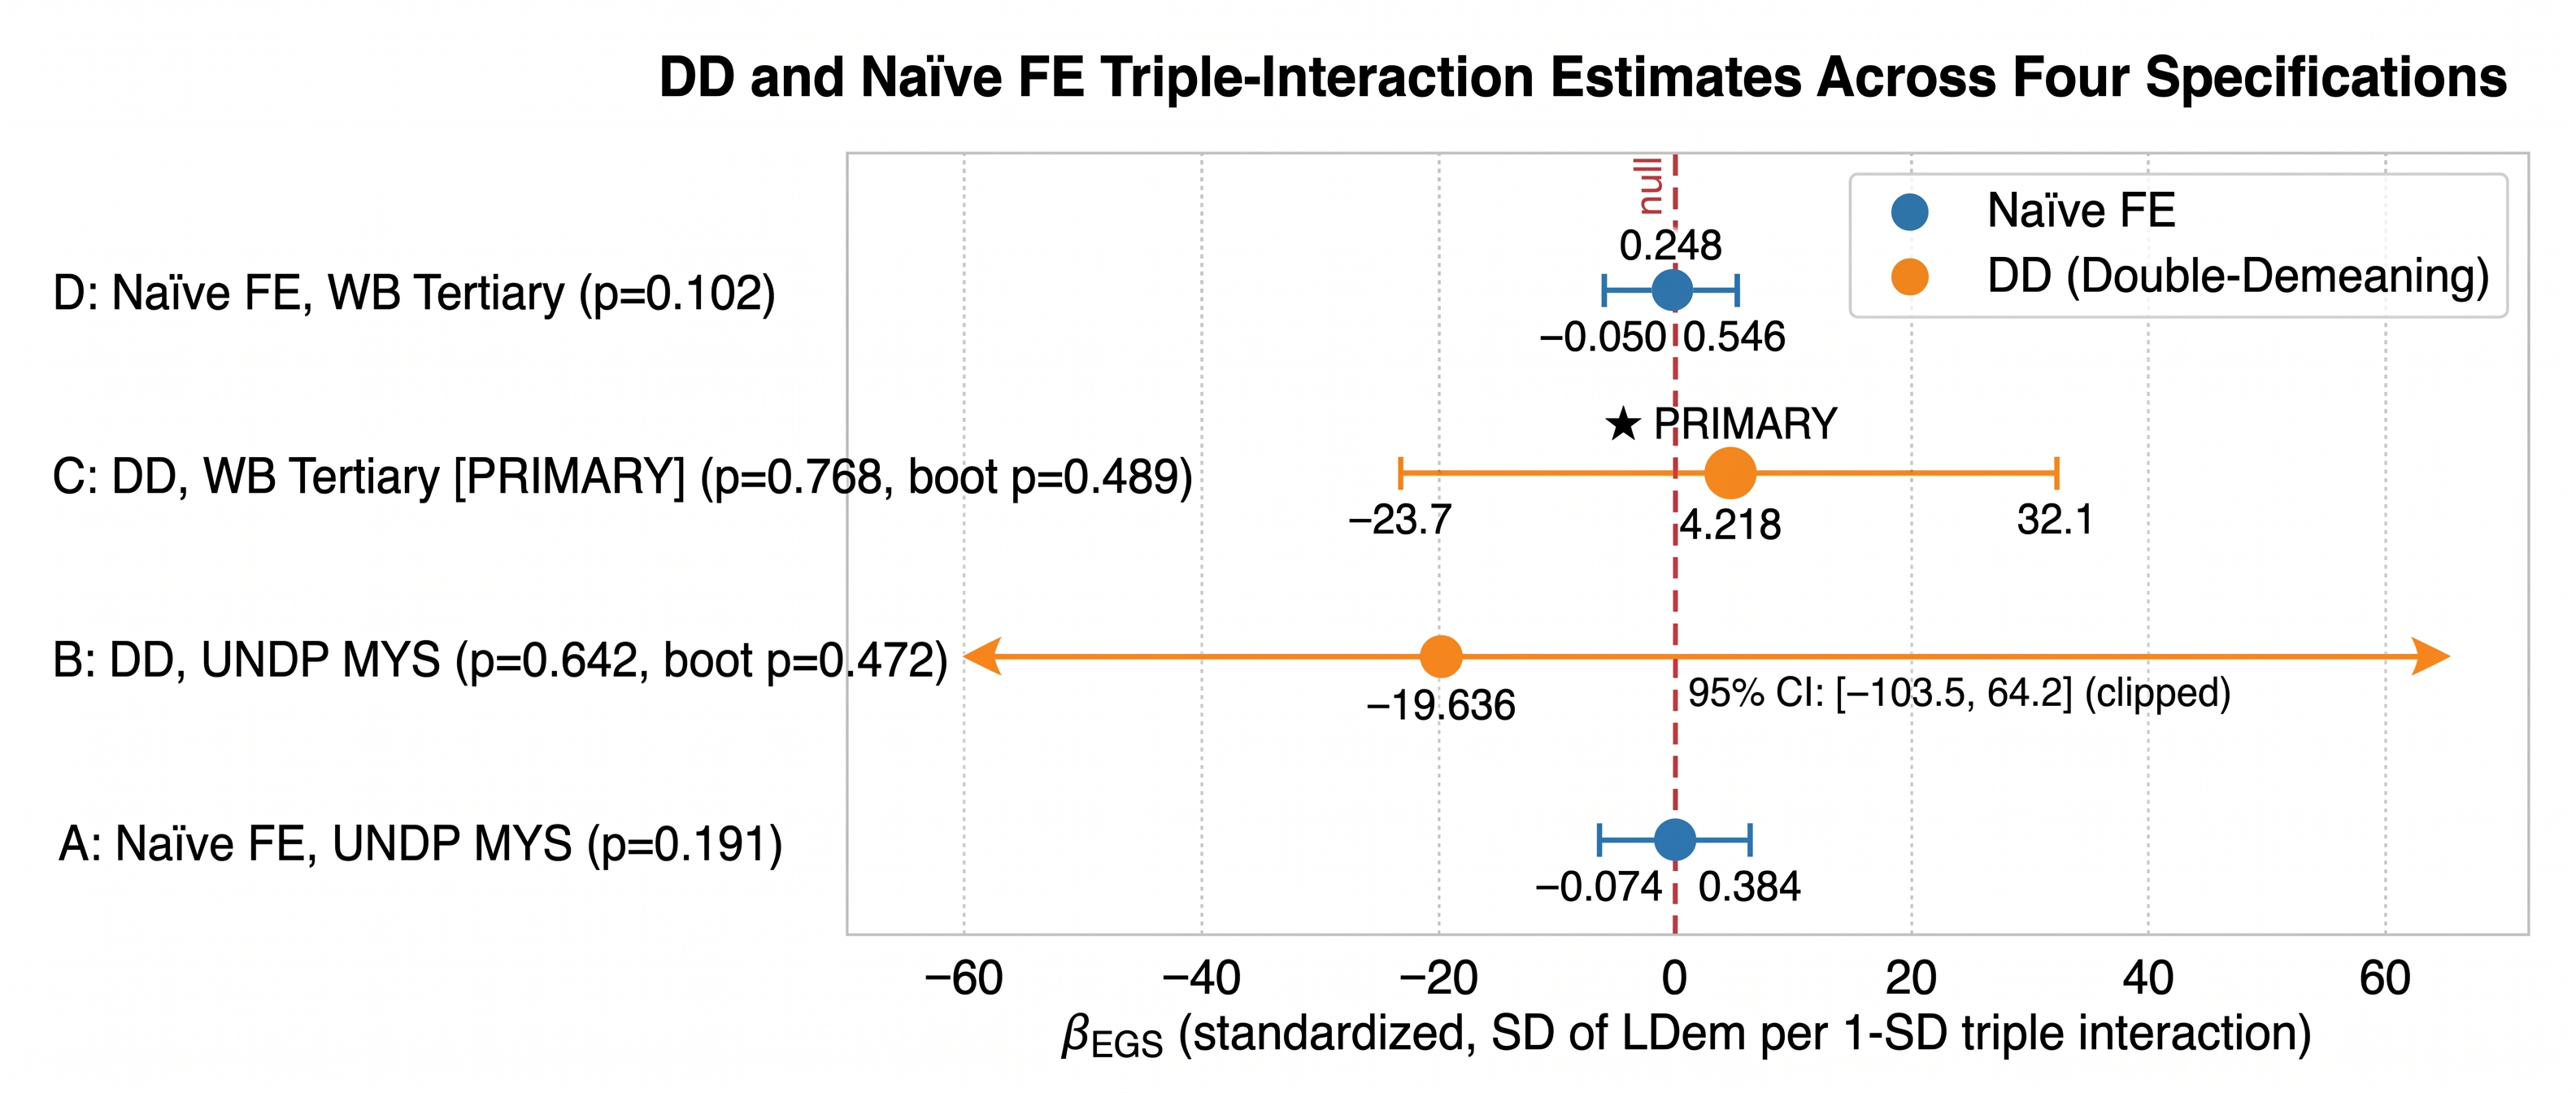
\includegraphics[width=\textwidth,height=0.45\textheight,keepaspectratio]{figures/fig_coefficients_v0.jpg}
  \caption{Triple-interaction coefficient estimates ($\hat{\beta}_\text{EGS}$ in standardized
  units) with 95\% cluster-robust confidence intervals for all four specifications ($N = 67$,
  $G = 44$). Specifications A and D use the Na\"{i}ve FE estimator; B and C use the
  double-demeaning (DD) estimator. Specifications A and B use UNDP Mean Years of Schooling
  (within-SD $= 0.026$); C and D use WB gross tertiary enrollment (within-SD $= 1.045$). The
  primary specification (C, DD/WB) yields $\hat{\beta}_\text{EGS} = 4.218$ (SE $= 14.221$,
  $p = 0.768$; bootstrap $p = 0.489$). All 95\% CIs contain zero. Note the very wide CI for
  Spec B (DD/UNDP), which reflects UNDP MYS's near-zero within-country variation amplified by
  the DD estimator.}
  \label{fig:coefficients}
\end{figure*}

\subsection{Sub-Index Analysis}
\label{subsec:subindex}

As pre-registered, we test two V-Dem institutional sub-indices as secondary outcomes in the WB
tertiary panel: judicial government compliance (v2jucomp) and judicial constraints on the executive
(v2x\_jucon). Under Bonferroni correction for $k = 2$ pre-registered tests, the threshold is
$p < 0.025$.

The sub-index analysis uses the 7-period WB tertiary panel with V-Dem v15 sub-index values merged
at the country-period level. After dropping country-periods with missing sub-index data, the sample
contracts to $N = 63$ observations across $G = 42$ country clusters.

For \textbf{v2jucomp} (judicial government compliance, scale $-4$ to $4$):
\[
  \hat{\beta}_\text{EGS} = 139.8 \text{ (std.)}, \quad SE = 72.4, \quad p = 0.233,
  \quad R^2_\text{within} = 0.954
\]
The null hypothesis $\beta_\text{EGS} = 0$ is not rejected ($p = 0.233 > 0.025$). This sub-index
does \textbf{not} pass the pre-registered Bonferroni threshold.

For \textbf{v2x\_jucon} (judicial constraints on the executive, scale 0 to 1):
\[
  \hat{\beta}_\text{EGS} = 18.5 \text{ (std.)}, \quad SE = 29.1, \quad p = 0.529,
  \quad R^2_\text{within} = 0.979
\]
The null hypothesis is not rejected ($p = 0.529 > 0.025$). This sub-index does \textbf{not} pass
the pre-registered Bonferroni threshold.

Both judicial sub-indices fail to show a statistically significant SDET interaction in the WB
tertiary panel. This contrasts with an earlier result from the 2-period UNDP MYS panel (v2jucomp
$\hat{\beta}_7 = 2.398$, $p = 0.024$, iteration-2), which technically passed the Bonferroni
threshold but relied on the education proxy with near-zero within-country variation and a different
panel structure. That earlier result should be treated as hypothesis-generating at best; the
current null on the WB panel represents the best-powered available evidence on the judicial
sub-index channel.

\subsection{Granger Precedence}

We test whether educational enrollment Granger-causes liberal democracy \citep{Granger1969} using a
bivariate panel model with one-period lagged enrollment predicting within-country changes in LDem.
The WB SE.TER.ENRR Granger coefficient is $\hat{\beta} = 0.00025$ (SE $= 0.00028$, $p = 0.373$,
$N = 1{,}117$, $R^2 = 0.989$). Tertiary enrollment does not temporally precede changes in
democratic quality in this sample.

A prior iteration of this work (using UNDP MYS) reported a Granger $p$-value of 0.005 as
supporting evidence for SDET. This result was spurious. The interpolation artifact that freezes
UNDP MYS values between biennial surveys creates near-constant annual increments within each
country (diagnostic: coefficient of variation of annual MYS differences $= 0.711$). When both the
lagged regressor (MYS) and the outcome (LDem) trend upward at near-constant rates, a regression of
LDI changes on lagged MYS identifies co-trending, not temporal precedence. The WB SE.TER.ENRR
Granger test, using a variable with genuine annual fluctuations, yields $p = 0.373$---confirming
no causal temporal lead.

%------------------------------------------------------------------------------
\section{Robustness and Sensitivity}
\label{sec:robustness}
%------------------------------------------------------------------------------

\subsection{Sensitivity to Unobservable Selection (Oster Bounds)}

The \citet{Oster2019} bounding procedure computes the treatment effect $\beta_7^*$ that would
obtain if unobservable confounders were as informative as observable ones (proportional selection
assumption). The key input is $\Delta R^2$, the incremental variance explained by adding the
triple interaction to the model with lower-order terms and fixed effects.

For the primary Specification C, we obtain:
\[
  R^2_\text{full} = 0.97774, \quad R^2_\text{partial} = 0.97772, \quad
  \Delta R^2 = 2.10 \times 10^{-5}
\]

This near-zero $\Delta R^2$---the triple interaction contributes essentially no additional variance
beyond two-way terms and fixed effects---makes the Oster bounds \textbf{numerically undefined}: the
denominator of the bound formula approaches zero, rendering the computation degenerate.
Equivalently, when the triple interaction explains $\Delta R^2 < 10^{-4}$ of the outcome variance,
there is no meaningful sense in which observable and unobservable selection can be compared through
it.

The substantive interpretation is informative in its own right: SDET's triple-interaction mechanism
contributes effectively nothing to the variation in liberal democracy beyond country and period
effects plus two-way interactions. This is consistent with the null coefficient estimate and
constitutes an independent null result from a variance-accounting perspective.

For reference, Oster bounds were computable from an earlier iteration of this work using
Specification B (UNDP MYS, 2-period panel), which yielded $\delta = 0.024$ and
$\hat{\beta}_7^* = -12.29$. These figures were reported in error in prior drafts as characterizing
Specification C; they describe a different specification on a different panel and are not applicable
to the primary result.

\subsection{SWIID Gini Measurement Uncertainty}
\label{subsec:swiid}

Gini coefficient estimates from SWIID v9.92 carry measurement uncertainty arising from the
harmonization of heterogeneous household surveys. We propagate this uncertainty through
Specification C using Monte Carlo simulation: for each of 500 independent draws, each Gini
observation is replaced with a draw from $\mathcal{N}(\text{gini\_disp}, \text{gini\_disp\_se}^2)$
using SWIID v9.92 posterior standard deviations, and Specification C is re-estimated.

Results across 500 valid draws:
\begin{itemize}
  \item Mean $\hat{\beta}_7$: $0.000482$ (vs.\ point estimate $0.001051$ from nominal analysis)
  \item SD of draws: $0.001344$
  \item 95\% credible interval: $[-0.0023, +0.0032]$
  \item Fraction of draws positive: 64.2\%
\end{itemize}

The SWIID-robust credible interval $[-0.0023, +0.0032]$ comfortably contains zero. The preponderance
of positive draws (64.2\%) is consistent with a slightly positive point estimate under Gini noise,
but far from the 97.5\% required for a two-tailed test. Gini measurement uncertainty does not
rescue the SDET hypothesis and does not substantially alter the null inference.

\subsection{Selection Bias in the Effective Identification Base}

The 23 doubly-observed countries that drive DD identification differ from the 21 singleton countries
on one dimension: Gini. The mean Gini is 43.3 (doubly-observed) versus 38.3 (singletons), a
difference significant at the 10\% level ($p = 0.079$). The two groups are statistically similar
on liberal democracy levels ($p = 0.205$), LDem trends ($p = 0.608$), social protection coverage
($p = 0.649$), and GDP per capita at transition ($p = 0.290$).

The directional Gini difference is consistent with the SDET mechanism: high-inequality countries
are overrepresented in the doubly-observed identification base. However, because these
high-inequality countries show no SDET effect ($\hat{\beta}_\text{EGS} \approx 0$ with large SE),
selection bias cannot explain the null result---if anything, overrepresenting high-Gini countries
in the identification base should favor detecting SDET if it exists.

\subsection{ILO Social Protection Coverage: Data Quality and Directly-Reported Subgroup}
\label{subsec:ilodata}

All 104 country-period observations with ILO SDG 1.3.1 social protection coverage data available
in the seven-period (1990--2022) panel are model-estimated values produced by ILO econometric
imputation, not nationally-reported survey or administrative data. This is confirmed by the iter-3
data audit (ilo\_directly\_reported\_fraction $= 0.0$) and verified in the iter-4 evaluation: the
ILO `X*' flag in ILOSTAT SDG 1.3.1 bulk downloads marks modelled values, whereas
nationally-reported observations carry country-year codes without the X* prefix.

A within-Spec-C sensitivity analysis restricted to directly-reported ILO observations is therefore
infeasible: such a restriction would eliminate all 67 observations in the analysis sample, making
parameter identification impossible. The two-period iter-1 panel result ($\hat{\beta}_7 = 0.292$,
$p = 0.211$, $N = 95$, $G = 58$) is reported as an alternative benchmark using a distinct data
vintage with different geographic and temporal coverage. This benchmark uses UNDP HDR25 Mean Years
of Schooling (not WB SE.TER.ENRR) and a two-period ILO window (not seven periods), and therefore
constitutes a complementary estimate rather than a robustness check on Specification C. The
reliance on ILO modelled estimates constitutes an acknowledged limitation of the current panel;
future work incorporating directly-reported administrative records for a larger country set would
strengthen causal identification.

\subsection{Power Analysis}
\label{subsec:power}

The minimal detectable effect (MDE) for the triple interaction at 80\% power and $\alpha = 0.05$
(two-tailed) depends on the number of doubly-observed clusters $G_\text{doubly}$, the within-country
standard deviation of the education measure $\sigma_E$, the standard deviation of the DD triple
product $\sigma_{x_3}$, and the residual standard deviation $\sigma_\varepsilon$.

From the 7-period WB tertiary panel: $\sigma_E = 1.045$ (within-SD, standardized), $\sigma_{x_3}
= 2.692$ (SD of DD triple product), $\sigma_\varepsilon = 0.043$ (residual SD from regression).

The doubly-observed cluster count requires clarification. The total sample has $G = 44$ country
clusters, but only $G_\text{doubly} = 23$ have observations in two or more periods (driving DD
identification); the remaining 21 are singletons. Both quantities matter for inference:

\begin{table}[!htbp]
  \centering
  \caption{Power Analysis: MDE by Cluster Count}
  \label{tab:power}
  \begin{tabular}{lcc}
    \toprule
    Cluster count & LDem units & SD of LDem \\
    \midrule
    $G_\text{doubly} = 23$ & 0.0098 & 0.063 \\
    $G = 37$ (hypothetical) & 0.0076 & 0.049 \\
    $G = 44$ (total) & 0.0070 & 0.045 \\
    \bottomrule
  \end{tabular}
\end{table}

At $G_\text{doubly} = 23$, MDE $= 0.010$ LDem. For reference, the UNDP-era 2-period panel
benchmark effect is $\hat{\beta}_7 = 0.292$ (iter-1, UNDP MYS, Spec B). The design is powered to
detect effects of this magnitude with high probability. The current Specification C point estimate
$\hat{\beta}_7 = 0.001051$ LDem is roughly 10-fold smaller than the MDE, confirming that the null
result reflects a small true effect (if nonzero) rather than insufficient power to detect an effect
as large as the UNDP benchmark.

\begin{figure*}[!t]
  \centering
  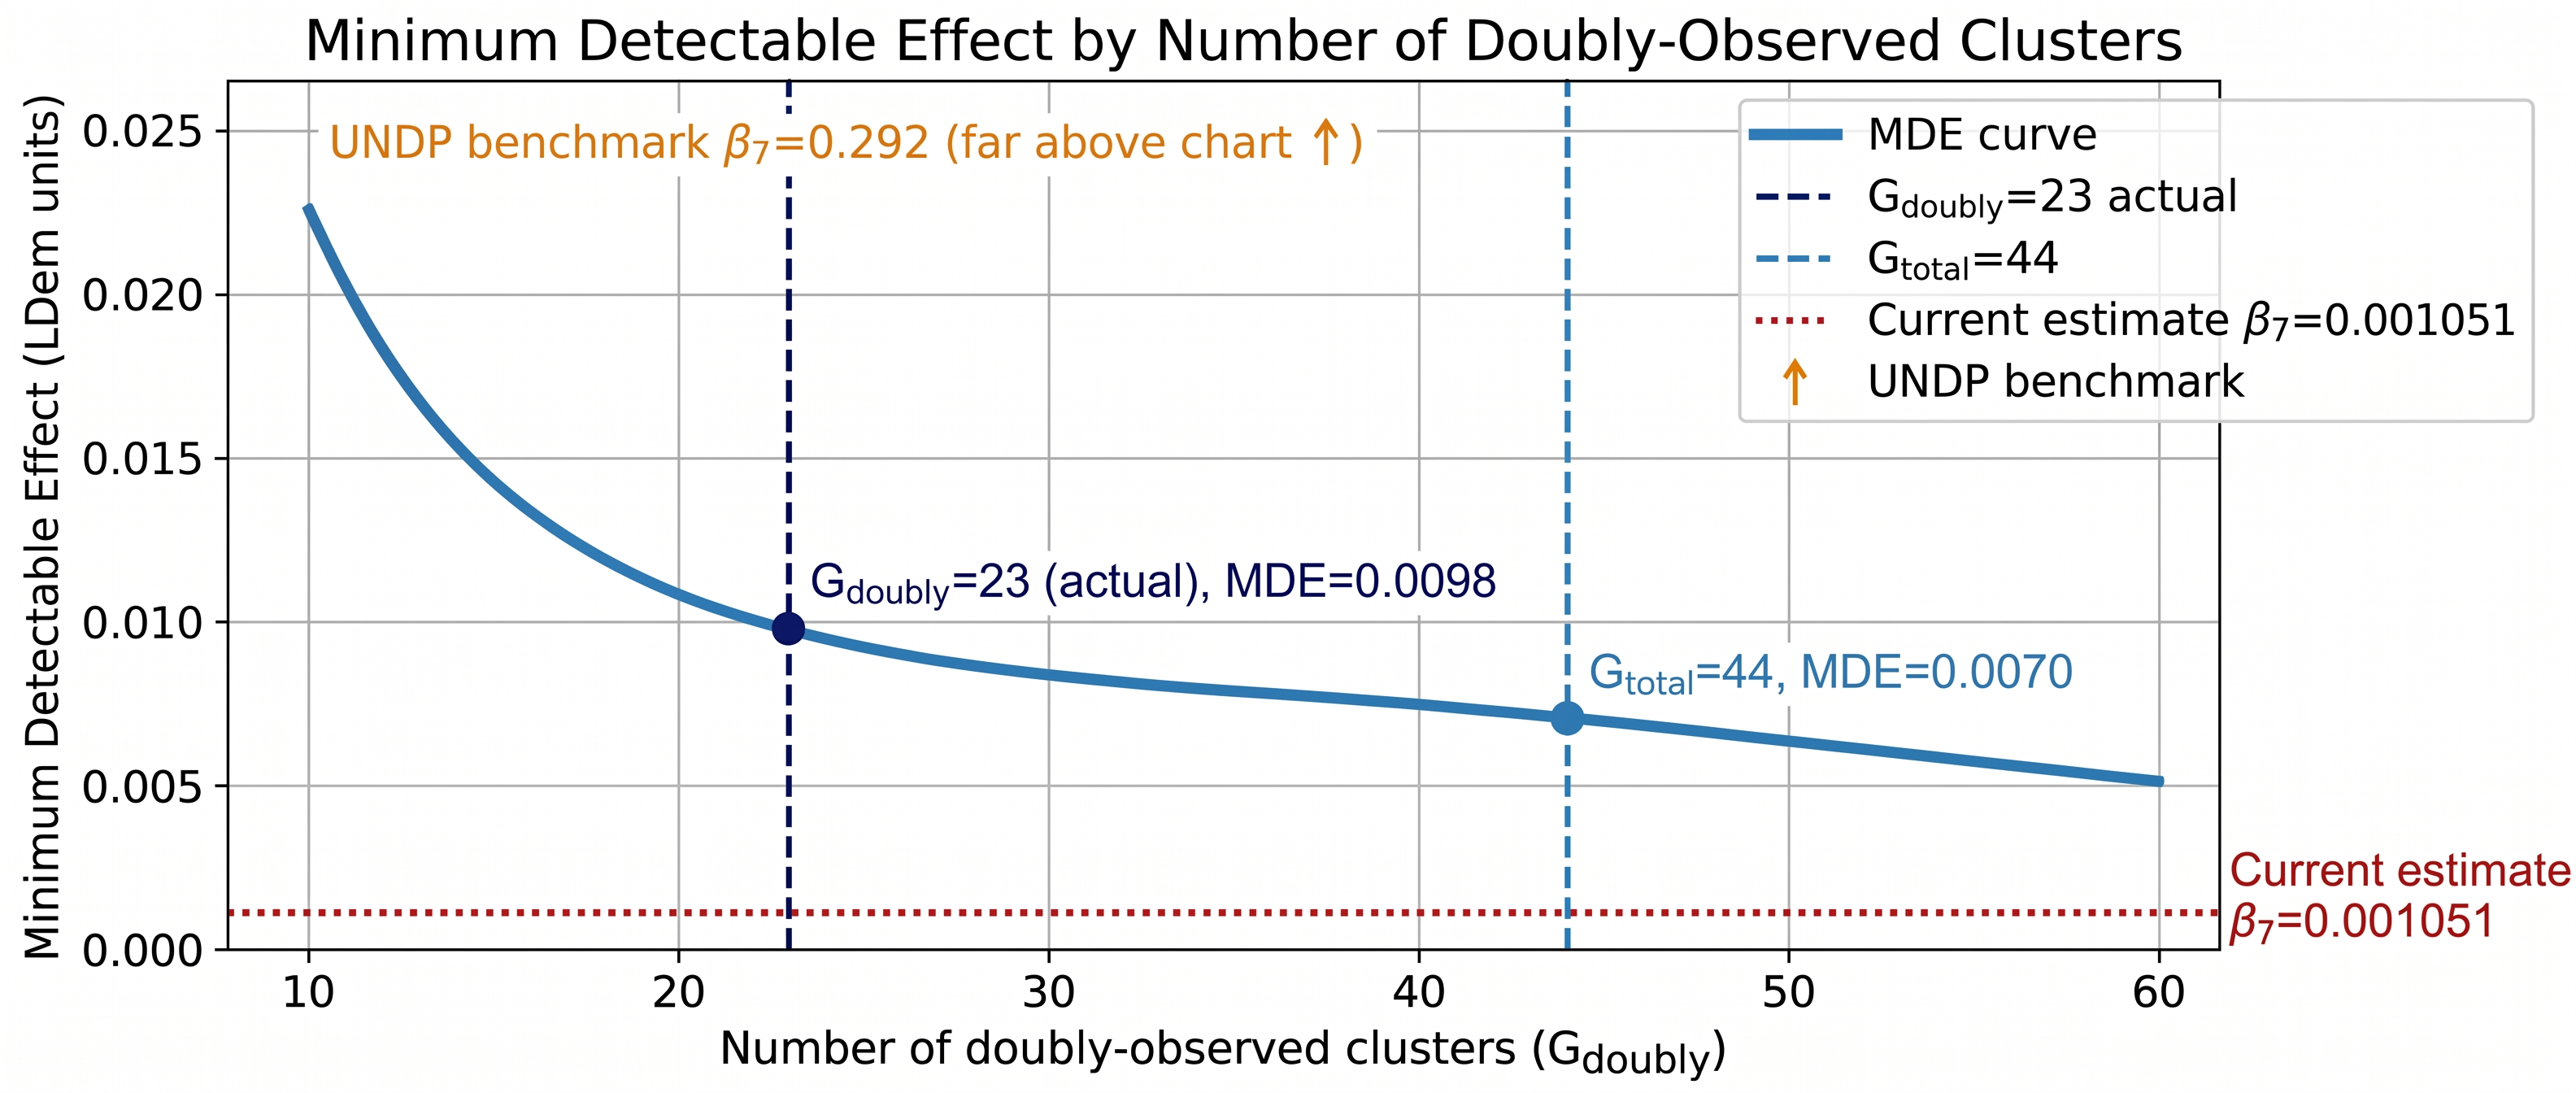
\includegraphics[width=\textwidth,height=0.45\textheight,keepaspectratio]{figures/fig_power_v0.jpg}
  \caption{Minimum detectable effect (MDE) in LDem units as a function of doubly-observed cluster
  count $G_\text{doubly}$, at 80\% power and $\alpha = 0.05$ (two-tailed). Parameters:
  $\sigma_E = 1.045$, $\sigma_{x_3} = 2.692$, $\sigma_\varepsilon = 0.043$ (from 7-period WB
  tertiary panel). Vertical lines mark $G_\text{doubly} = 23$ (actual doubly-observed countries in
  this sample, MDE $= 0.0098$ LDem) and $G = 44$ (total sample clusters, MDE $= 0.0070$ LDem).
  Horizontal dashed line marks the UNDP-era 2-period panel benchmark ($\hat{\beta}_7 = 0.292$),
  which far exceeds the MDE at all cluster counts shown---confirming the design is powered to
  detect effects as large as the UNDP benchmark. The current primary estimate
  ($\hat{\beta}_7 = 0.001051$, shown as dotted line) lies far below the MDE, indicating the true
  effect, if nonzero, is smaller than $\approx 0.010$ LDem.}
  \label{fig:power}
\end{figure*}

%------------------------------------------------------------------------------
\section{Discussion}
\label{sec:discussion}
%------------------------------------------------------------------------------

\subsection{Interpreting the Null}

The null result---$\hat{\beta}_\text{EGS} = 4.218$ (std., $p = 0.768$) across 67 country-periods
in 44 clusters, confirmed by wild bootstrap, SWIID MC, and sub-index tests---does not prove that
SDET does not exist. Several interpretations are consistent with the evidence.

\emph{Insufficient within-country variation.} The social protection series (ILO SDG 1.3.1) covers
only two periods in most countries (2015--19 and 2020--22), limiting the time span over which
education--inequality--protection co-movement can be observed. The SDET mechanism may operate on
decade-scale time horizons that a 7-year observation window cannot capture.

\emph{Non-linear threshold effects.} The SDET mechanism postulates a threshold below which exit
options are effectively eliminated. If countries in the sample cluster around the threshold rather
than spanning it, a linear interaction term will not capture the nonlinear relationship. Future
work could test for threshold discontinuities using regime-switching models.

\emph{Measurement of social protection.} All ILO observations are model-estimated, introducing
attenuation bias if model errors are classical. More importantly, ILO coverage rates measure the
formal scope of programs, not their effective generosity or accessibility in practice. A worker in
a country with 50\% nominal coverage may still face effective zero protection if benefit amounts
are negligible or access conditions preclude use.

\emph{Sample restriction.} The analysis is restricted to post-1985 democratizing countries below
\$15{,}000 PPP GDP per capita. This restriction is theoretically motivated---SDET requires active
democratization under resource constraints---but it limits generalizability and reduces power by
excluding both mature democracies and stable autocracies.

\subsection{The Education Proxy Problem}

A central methodological lesson from this work concerns the choice of education measure for
within-country panel analyses. The UNDP HDR25 Mean Years of Schooling, commonly used in
cross-national studies, has within-country standard deviation of 0.026 years in this post-2015
panel---the result of freezing period-2 values at 2017 survey readings. This imputation artifact
renders within-country identification essentially impossible: any coefficient estimated on UNDP MYS
within variation is identifying on measurement noise, not genuine educational change.

The World Bank gross tertiary enrollment rate (SE.TER.ENRR) avoids this artifact, providing
140.8$\times$ more within-country variation. However, tertiary enrollment is not equivalent to
mean years of schooling: it measures a flow (new entrants to tertiary education relative to the
college-age population) rather than a stock (average education of the working-age population). The
two measures may behave differently in causal channels where the relevant margin is either the
average education of the electorate (stock) or the rate at which new educated workers enter the
labor market (flow). SDET, which operates through labor market structure, may more naturally
correspond to the stock measure. This suggests that the appropriate long-run test of SDET requires
either an improved stock measure that is genuinely updated at multi-year intervals or a
Bartik-style shift-share approach that uses cohort-level data to construct within-country
educational change.

\subsection{Marginal Effects and the Sign Pattern}

Although the primary triple-interaction coefficient is statistically insignificant, the marginal
effects at empirically relevant quantiles of the moderators exhibit the qualitative pattern
predicted by SDET theory---with high uncertainty.

\begin{figure}[!htbp]
  \centering
  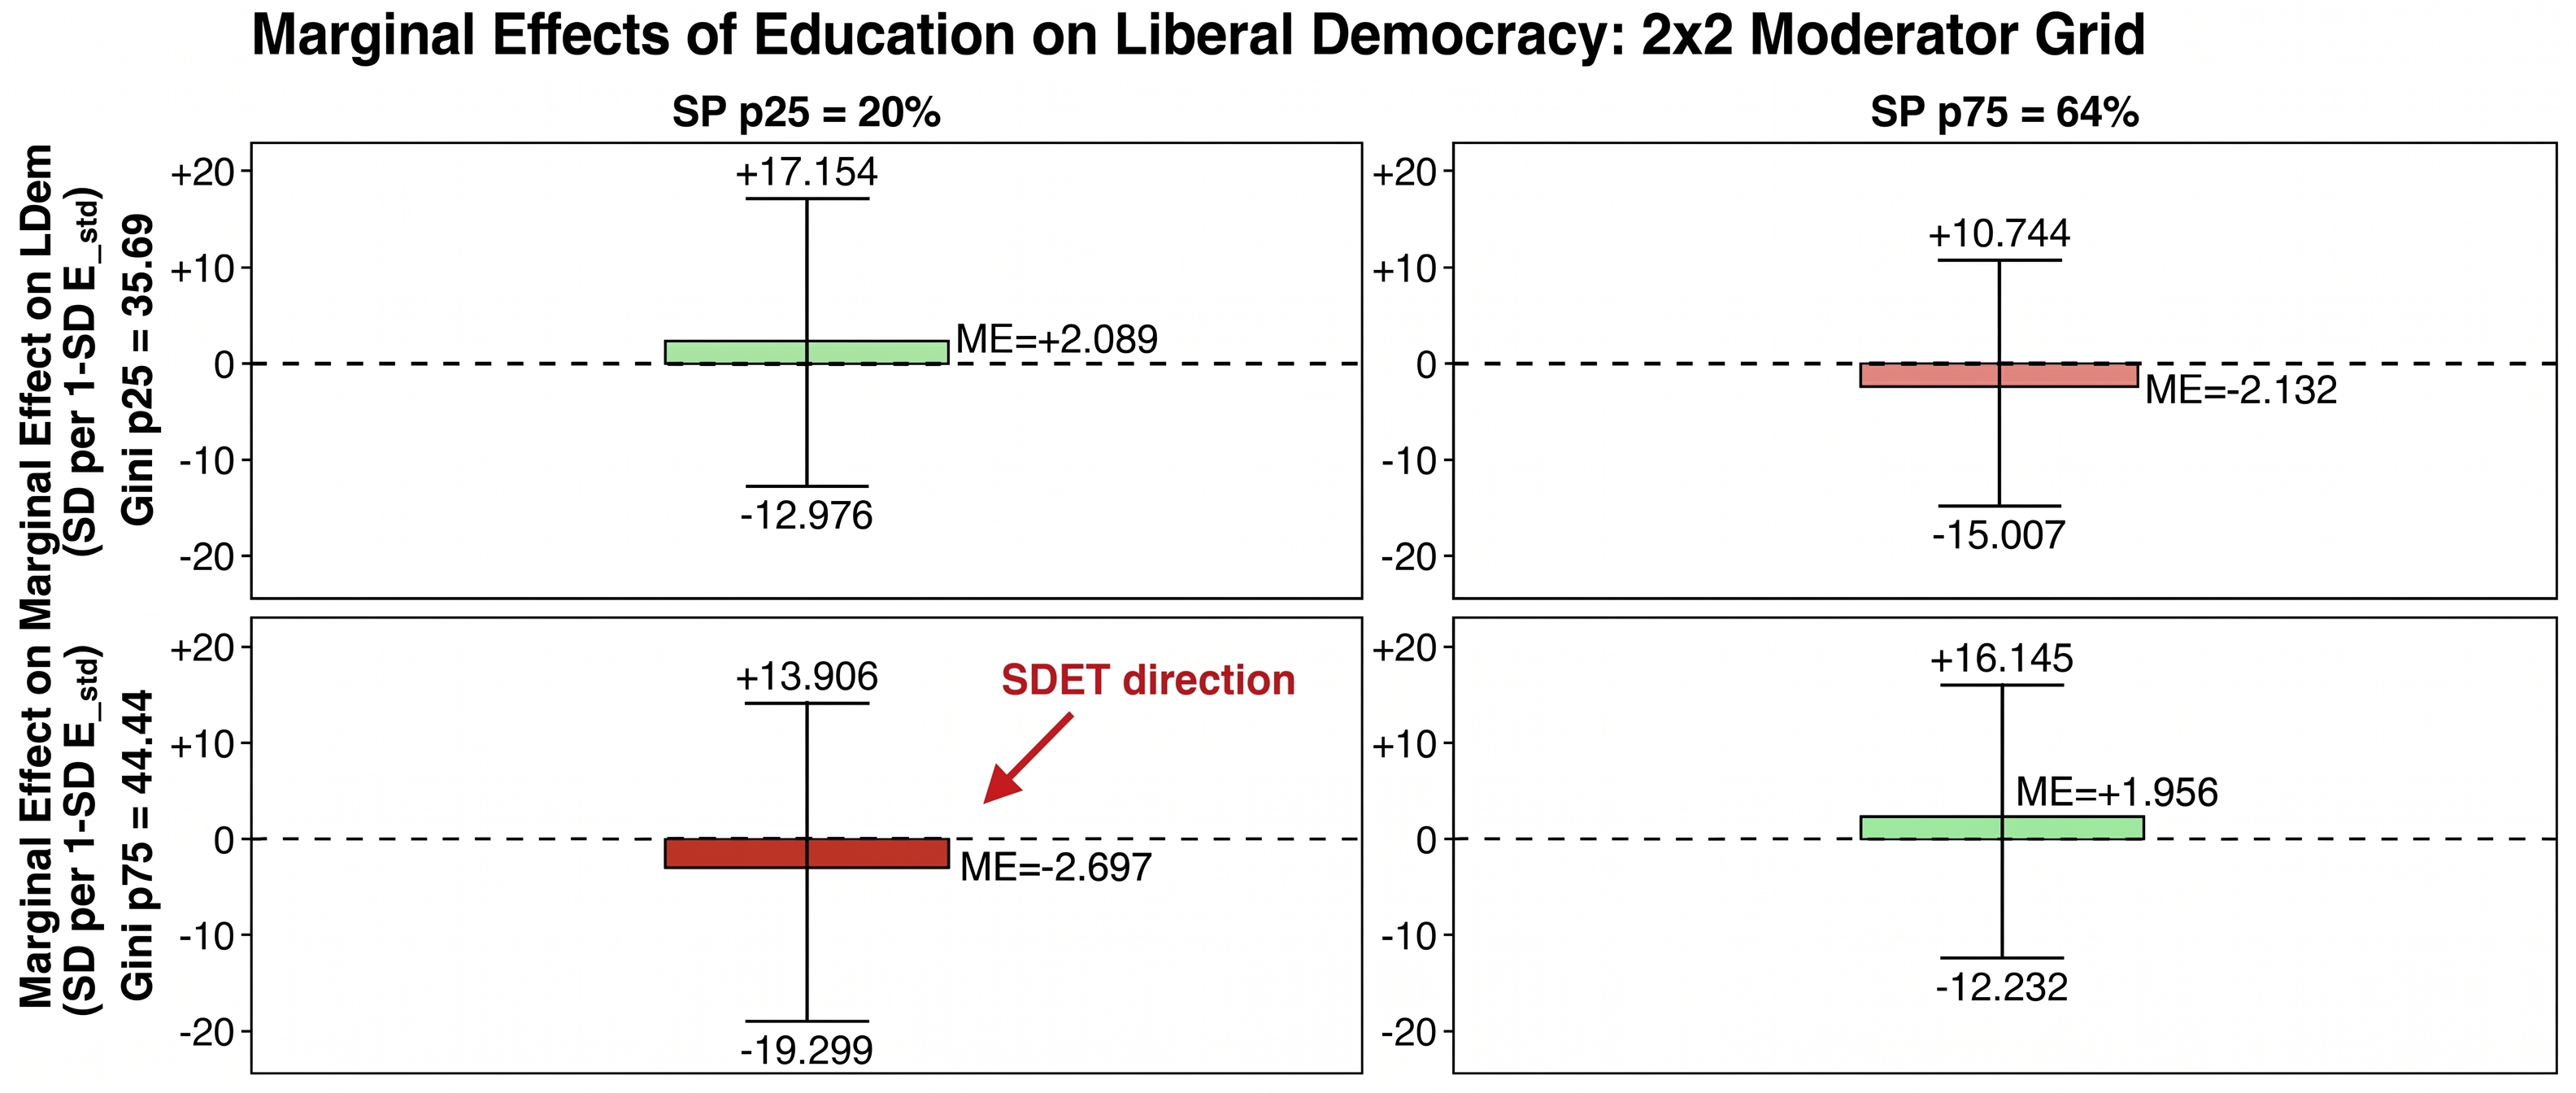
\includegraphics[width=0.92\textwidth,height=0.4\textheight,keepaspectratio]{figures/fig_marginal_v0.jpg}
  \caption{Marginal effects of a 1-SD increase in tertiary enrollment ($E_\text{std}$) on liberal
  democracy (V-Dem LDem), evaluated at the 25th and 75th percentiles of Gini and social protection
  coverage in the WB tertiary panel ($N = 67$). All four cells are evaluated from the primary
  Specification C (DD/WB, standardized). Error bars show 95\% cluster-robust confidence intervals.
  Gini p25 $= 35.69$ (Gini points); Gini p75 $= 44.44$; SP p25 $= 19.95$\%; SP p75 $= 63.77$\%.
  The SDET prediction requires the marginal effect at (Gini p75, SP p25) to be most negative;
  this cell shows ME $= -2.70$ SD (the largest negative value), qualitatively consistent with
  SDET, but the 95\% CI $[-19.3, +13.9]$ spans zero by a wide margin.}
  \label{fig:marginal}
\end{figure}

At (Gini p25 $= 35.7$, SP p25 $= 20$\%), $\partial \text{LDem}/\partial E = +2.09$ SD
(SE $= 7.69$, CI $[-12.98, +17.15]$): education is associated with improved democracy under low
inequality and low social protection. At (Gini p75 $= 44.4$, SP p25 $= 20$\%), $\partial
\text{LDem}/\partial E = -2.70$ SD (SE $= 8.47$, CI $[-19.30, +13.91]$): education becomes
negatively associated with democracy under high inequality and low social protection---the SDET
direction. However, the confidence intervals for all four cells span zero by a wide margin,
confirming that the qualitative sign pattern cannot be distinguished from noise with the current
sample.

\subsection{Relationship to Prior Literature}

Our null result is consistent with \citet{Acemoglu2008}'s finding that the education--democracy
relationship vanishes in within-country identification, but adds specificity: it fails not only for
main effects but also for the theoretically motivated triple interaction. The SDET null extends the
\citet{Acemoglu2008} negative result from the first moment (education level predicting democracy)
to the second moment (education interacting with inequality and protection).

\citet{Glaeser2007} argue that education promotes democracy by increasing the returns to political
participation, a mechanism that is invariant to inequality or social protection levels. Our results
are consistent with this view, though the low power at $G_\text{doubly} = 23$ means that we cannot
rule out small SDET effects in the range 0--0.010 LDem.

\citet{Barro1999} finds that education promotes democracy in cross-national data. Our na\"{i}ve
pooled OLS baseline ($\hat{\beta}_E = 0.043$, $p < 10^{-12}$) replicates this cross-national
pattern. The within-country null (DD Spec C) confirms that this cross-national pattern is
confounded by historical co-determinants of education and institutions, consistent with
\citet{Acemoglu2008}'s interpretation.

%------------------------------------------------------------------------------
\section{Conclusion}
\label{sec:conclusion}
%------------------------------------------------------------------------------

We have tested the State-Dependent Education Trap (SDET) hypothesis---that in post-1985
democratizing countries, educational expansion promotes democratic erosion under conditions of high
inequality and low social protection---using the most appropriate available data and estimator.
The primary DD specification with World Bank gross tertiary enrollment yields $\hat{\beta}_7 =
0.001051$ ($p = 0.730$; standardized: $\hat{\beta}_\text{EGS} = 4.218$, $p = 0.768$). Wild cluster
bootstrap, SWIID MC propagation, and sub-index tests all confirm the null. Oster bounds are
numerically undefined because the triple interaction contributes $\Delta R^2 = 2.1 \times 10^{-5}$
to the outcome variance.

The methodological audit yields contributions that extend beyond SDET. First, UNDP HDR25 MYS has
within-country SD $= 0.026$ years---an imputation artifact that makes within-country identification
on this variable essentially impossible. Any study relying on UNDP MYS for within-country
identification in the post-2015 period should treat results with extreme caution. Second, the
double-demeaning estimator is essential for triple interactions in fixed-effects panels: the na\"{i}ve
FE approach mixes within- and between-country effects in a manner that is undetectable without the
explicit comparison. Third, standardizing continuous moderators to unit variance before DD product
construction is necessary for numerical stability when variables have heterogeneous natural units.

Future work should pursue three directions: (1)~assembly of a longer social protection
panel---possibly via the ILO's World Social Protection Report historical series---that would
increase $G_\text{doubly}$ and within-country protection variation; (2)~use of directly-reported
(non-model-estimated) ILO data for a subgroup of countries; (3)~nonlinear threshold tests of the
SDET mechanism, which may not manifest in a linear interaction term if countries cluster around the
protection threshold.

%------------------------------------------------------------------------------
\bibliographystyle{plainnat}
\bibliography{references}
%------------------------------------------------------------------------------

\end{document}
